% \subsection{Stability and Equilibrium Points}

% \subsubsection{Equilibrium Points}

% Given the system:

% $$
% \begin{cases}
%     \dot x = f(x) \\
%     x \in \mathbb{R}^n
% \end{cases}
% $$

% An equilibrium point is a point $x^*$ such that $f(x^*) = 0$.

% \begin{tipsblock}[Eq. points]
% A system can have multiple equilibrium points.
% \end{tipsblock}

% We have three kinds of equilibrium:

% \begin{itemize}
%     \item \textbf{Stable equilibrium}: if the system is in the neighborhood of the equilibrium point, it will remain there.
%     \item \textbf{Neutral equilibrium}: if the system is in the neighborhood of the equilibrium point, it will remain there, but it will not return to it.
%     \item \textbf{Unstable equilibrium}: if the system is in the neighborhood of the equilibrium point, it will move away from it.
% \end{itemize}

% \begin{figure}[H]
%     \centering
%     \includegraphics[width=0.65\textwidth]{assets/eq_points.png}
%     \caption{Stable, Natural and Unstable Equilibrium Points \cite{stability}}
% \end{figure}

% \subsubsection{Stability}

% We say that a system is \textbf{\textit{Globally Asymptotically Stable}} (or \textit{Globally Attractive}) if it is stable and if it converges to the equilibrium point from any initial condition.

% \subsection{Local Analysis Near the Equilibrium Point}

% In this section, we study the system in the neighborhood of the equilibrium point. Let the initial condition be a small perturbation around the equilibrium:

% $$
% X(0) = X_e + \varepsilon.
% $$

% We introduce a deviation function $U(t)$ defined by

% $$
% X(t) = X_e + U(t),
% $$

% with the initial condition

% $$
% U(0) = \varepsilon.
% $$

% Thus, the evolution of the perturbation is governed by

% $$
% \begin{cases}
% \dot U = f(X_e + U), \\
% U(0) = \varepsilon.
% \end{cases}
% $$

% Assume that the dynamics of the system are given by

% $$
% \dot X = X(b(X) - m(X)).
% $$

% Then the perturbed system becomes

% $$
% \dot U = (b(X_e + U) - m(X_e + U))(X_e + U).
% $$

% Expanding $b(X_e + U)$ and $m(X_e + U)$ in a Taylor series around $X_e$, we have:

% $$
% b(X_e + U) \approx b(X_e) + b'(X_e)U,
% $$
% $$
% m(X_e + U) \approx m(X_e) + m'(X_e)U.
% $$

% Substituting these into the equation for $\dot U$, we get:

% $$
% \begin{array}{rl}
% \dot U & = \bigl[b(X_e) + b'(X_e)U\bigr] - \bigl[m(X_e) + m'(X_e)U\bigr](X_e + U) \\
%       & = \bigl[b(X_e) + b'(X_e)U\bigr] - \bigl[m(X_e)X_e + m(X_e)U + m'(X_e)X_eU + m'(X_e)U^2\bigr].
% \end{array}
% $$

% Since the equilibrium condition implies that

% $$
% (b(X_e) - m(X_e))X_e = 0,
% $$

% the above expression simplifies (neglecting the higher-order term $m'(X_e)U^2$) to:

% $$
% \dot U \approx \left[b'(X_e) - m(X_e) - m'(X_e)X_e\right] U.
% $$

% Under the assumption that $b'(X_e)$ is negative, we can express this as

% $$
% \dot U \approx -X_e\Bigl(|b'(X_e)| + m'(X_e)\Bigr)U.
% $$

% The solution of this linearized differential equation is given by:

% $$
% U(t) = U(0)\,e^{-X_e (|b'(X_e)| + m'(X_e))t}.
% $$

% Hence, we identify the decay rate (or the inverse of the characteristic time constant) as

% $$
% X_e\Bigl(|b'(X_e)| + m'(X_e)\Bigr),
% $$

% and the characteristic time $\tau$ is:

% $$
% \tau = \frac{1}{X_e \left(|b'(X_e)| + m'(X_e)\right)}.
% $$

% This time constant represents the rate at which perturbations decay in the vicinity of the equilibrium point.


% \newpage

% $$
% X(t) = X_e + U(t) \Rightarrow \dot U = f(X_e + U) = \underbrace{f(X_e)}_{=\ 0} + f'(X_e)U + O(U^2)
% $$

% $$
% \dot U = f'(X_e)U \Rightarrow U(t) = U(0) e^{f'(X_e)t}
% $$

% So we have:
% $$
% \begin{cases}
% f'(X_e) < 0 \quad \Rightarrow \quad X_e \text{ is Locally Asintotically stable } \\
% f'(X_e) > 0 \quad \Rightarrow \quad X_e \text{ is Unstable }
% \end{cases}
% $$

% \vspace{2em}

% \section{Non-scalar Systems}

% Consider the system:

% $$
% \begin{cases}
%     \dot x = f(x) \\
%     x \in \mathcal{f} \subseteq \mathbb{R}^n
% \end{cases}
% $$

% As in the scalar case, we can linearize the system around the equilibrium point $x_e$:

% $$
% f(X_e) = 0
% $$

% $$
% X = X_e + U, \quad \quad |U| \ll 1
% $$

% We have to consider the Jacobian matrix of $f$:

% \dots

% \subsection{Exponential of a Matrix}

% Let's consider a linear system of the form:

% $$
% \dot x = Ax
% $$

% where $A \in \mathbb{R}^{n \times n}$ is a matrix. The solution of this system is given by:

% $$
% x(t) = e^{At} x(0)
% $$

% where $e^{At}$ is the exponential of the matrix $A$.

% \begin{definitionblock}[Exponential of a Matrix]
% Given a matrix $A \in \mathbb{R}^{n \times n}$, the exponential of $A$ is defined as:

% $$
% e^A = I + A + \frac{A^2}{2!} + \frac{A^3}{3!} + \dots = \sum_{k=0}^{\infty} \frac{A^k}{k!}
% $$

% This comes from the Taylor series expansion of the exponential function.
% \end{definitionblock}

% $$
% \dfrac d{dt} e^{At} = \sum_{m = 1}^\infty A^m m \dfrac{t^{m-1}}{m(m-1)!}
% = \sum_{k = 0}^\infty A A^k \dfrac{t^k}{k!}
% = A e^{At}
% $$

% $$
% \begin{array}{lll}
% A & = & H \cdot \text{Diag}(\lambda_1, \lambda_2, \dots, \lambda_n) \cdot H^{-1} \\
% A^2 & = & H \cdot \text{Diag}(\lambda_1^2, \lambda_2^2, \dots, \lambda_n^2) \cdot H^{-1} \\
% A^m & = & H \cdot \text{Diag}(\lambda_1^m, \lambda_2^m, \dots, \lambda_n^m) \cdot H^{-1}
% \end{array}
% $$

% So we have:

% $$
% e^{At} = \sum_{m = 0} ^ \infty \dfrac{A^m t^m}{m!} = 
% $$

\chapter{Stochastic Numerical Methods}

The non-differentiability of the Wiener process path fundamentally breaks the foundation of classical calculus, rendering traditional analytical techniques inadequate for stochastic differential equations. This mathematical obstacle necessitates the development of an entirely new framework—stochastic calculus, with its own integration theory and differentiation rules.

\vspace{-0.7em}

\section{The Differential Form of SDEs: Itô Equation}

Let's reconsider Newton's second law. In its most common form, it is written as $F=ma$. However, its more fundamental statement relates force to the change in momentum $p=mv$, expressed in differential form as:
$$
dp = F dt
$$
This form is more general. For instance, consider the motion of a rocket, whose mass $m(t)$ changes as it consumes fuel. In this case, $F=ma$ is incorrect. The correct formulation is:
$$
d(m(t)v(t)) = F dt
$$
This differential way of writing physical laws is powerful and provides the foundation for correctly interpreting stochastic equations. A Langevin equation written as $\dot{x} = f(x,t) + g(x,t)\xi(t)$ is mathematically problematic. The rigorous approach is to express it in its differential form using the Wiener process increment $dW_t$, which represents the integral of the white noise $\xi(t)$:
$$
dx = f(x,t)dt + g(x,t)dW_t
$$
This is a \textbf{Stochastic Differential Equation (SDE)}. Its solution is understood in an integral sense:
$$
x(t) = x_0 + \int_0^t f(x(\tau), \tau)d\tau + \int_0^t g(x(\tau), \tau)dW_\tau
$$
The second integral is a stochastic integral, an object whose properties are fundamentally different from the standard Riemann integral. The infinitesimal increment $dW_t$ is defined as $dW_t = W(t+dt) - W(t)$. As we have established, it is a Gaussian random variable with mean 0 and variance $dt$, so $dW_t \sim \mathcal{N}(0, dt)$. This can be expressed as:
$$
dW_t = G(t)\sqrt{dt}
$$
where $G(t)$ is a random variable drawn from the standard normal distribution, $\mathcal{N}(0,1)$.

The stochastic integral $\int_0^t g(x(\tau), \tau)dW_\tau$ represents the cumulative effect of the random forcing over time. Unlike deterministic integrals, this integral cannot be evaluated using traditional calculus rules due to the irregular nature of the Wiener process paths. The integral must be understood in the sense of Itô or Stratonovich, with Itô integration being the more commonly used convention in stochastic differential equations.

\begin{definitionblock}[Itô Equation]
Given an SLAE, we can always rewrite it as an \textbf{Itô equation}, by defining $dW = G(t)\sqrt{dt}$:
$$
dx = f(x)dt + g(x)dW
$$
\end{definitionblock}

\subsection{The Euler-Maruyama Method}

The Itô equation can be solved numerically using the Maruyama algorithm for stochastic differential equations. This is essentially the stochastic version of Euler's algorithm. Given a time interval $[0, T]$ and $h = T/N$, so that $t = jh$ for $j = 0, \ldots, N$. Suppose the Euler algorithm is:
$$
dx = x(t_j + h) - x(t_j) = x(t_{j+1}) - x(t_j)
$$
we can set $dt \approx h$ and write:
$$
x(t_{j+1}) = x(t_j) + f(x(t_j))h
$$

The Maruyama formula starts from this form by also considering the Gaussian effect, adding:
$$
x(t_{j+1}) = x(t_j) + f(x(t_j))h + G_j\sqrt{h}
$$
with $G_j \sim \mathcal{N}(0,1)$. Obviously, starting from this algorithm, more precise variants have been successively created.

\begin{definitionblock}[The Euler-Maruyama Method]
For the stochastic differential equation $dX_t = a(X_t, t)dt + b(X_t, t)dW_t$ with initial condition $X(0) = x_0$ and uniform time step $h$, the Euler-Maruyama approximation is given by:
$$
X_{j+1} = X_j + a(X_j, t_j)h + b(X_j, t_j)\sqrt{h}G_j
$$
where $t_j = jh$ and $\{G_j\}_{j=0}^{N-1}$ is a sequence of independent standard normal random variables.
\end{definitionblock}

This numerical scheme provides a practical foundation for simulating stochastic processes, though more sophisticated methods have been developed to improve accuracy and stability for specific applications.

\subsection{Itô's Lemma: The Stochastic Chain Rule}

Having established the framework of Itô equations, we now turn our attention to the fundamental problem of change of variables in stochastic calculus. When dealing with deterministic differential equations, the chain rule provides a straightforward mechanism for transforming variables. However, in the stochastic setting, the irregular nature of Brownian motion necessitates a more sophisticated approach.

Consider an SDE in Itô form:
$$
dx = a(x)dt + b(x)dW
$$
Suppose we wish to perform a transformation from $x$ to $y$ defined by $y = \psi(x)$. Our objective is to derive an equation of similar form for the transformed variable $y$.

Following the classical approach, we expand $dy$ in a Taylor series:
$$
\begin{array}{rl}
dy & = \psi'(x)dx + \frac{1}{2}\psi''(x)(dx)^2 + \ldots \\
& = \Psi'(x)[a(x)dt + b(x)dw] + \dfrac 12 \Psi''(x)
\left[
    b^2(x)(dw)^2 +
    \underbrace{\cancel{a^2(x)(dt)^2}}_{O(dt^2)} +
    \underbrace{\cancel{2a(x)b(x)dt dw}}_{O(dt^{3/2})}
\right]
\end{array}
$$

To derive a formula consistent with the Itô framework, we must carefully consider the order of magnitude of each term. Since $dW = O(\sqrt{dt})$, we can eliminate terms of order $(dt)^{3/2}$ and higher, including the mixed term $dt\,dW$ and $(dt)^2$. The remaining term $(dW)^2$ is of order $dt$, and by the fundamental property of Brownian motion, we have $(dW)^2 = dt$. 

Substituting this, we get:
$$
dy = \psi'(x)a(x)dt + \psi'(x)b(x)dW + \frac{b(x)^2}{2}\psi''(x)dt
$$

Realigning the terms, we get:
$$
dy = \left[\psi'(x)a(x) + \frac{b(x)^2}{2}\psi''(x)\right]dt + \psi'(x)b(x)dW
$$

\begin{definitionblock}[Itô's Lemma]
Let $X_t$ be an Itô process that satisfies the SDE $dX_t = a(X_t, t)dt + b(X_t, t)dW_t$. Let $\psi(x,t)$ be a twice-differentiable scalar function. Then the process $Y_t = \psi(X_t, t)$ is also an Itô process, and its differential $dY_t$ is given by:
$$
dY_t = \left[ \psi'(x)a(x) + \psi''(x)\frac{b(x)^2}{2} \right]dt + \psi'(x)b(x)dW_t
$$
\end{definitionblock}

This fundamental result encompasses the classical chain rule terms, namely $\psi'a$ and $\psi'b$, augmented by an additional stochastic correction term, $\psi''\frac{b^2}{2}$, known as the \textbf{Itô correction}. This correction term arises directly from the non-vanishing quadratic variation of the Wiener process and represents the fundamental distinction between stochastic and deterministic calculus.

\section{The Stochastic Malthusian Model and its Paradox}

The simplest model of population growth is the Malthusian model, which assumes an unlimited environment and a constant per capita growth rate, $r$. The dynamics are described by the ODE:
\vspace{0.4em}
$$
\dot{x} = rx
$$
where $x(t)$ represents the population size. The solution is simple exponential growth or decay, $x(t) = x(0)e^{rt}$. A more realistic model acknowledges that the growth rate is not constant but fluctuates randomly due to environmental variations. We can model this by making the growth rate a stochastic process, $r \to r + \omega\xi(t)$. This leads to the \bfit{stochastic Malthusian model}, an SDE with multiplicative noise:
$$
dx = (r + \omega\xi(t)) x
$$
where $\omega$ denotes the multiplicative noise amplitude. We can obtain the Ito formula:
$$
dx = rx\dd t + \omega x \dd W
$$
The solution of this stochastic equation can be obtained by applying Itô's formula. Setting $y = \ln x$, we find the drift and diffusion coefficients for the transformed process. Using Itô's rule:
\small
$$
dy = \left[ \frac{1}{x}rx - \frac{1}{2x^2}\omega^2 x^2 \right] \dd t + \dfrac 1x \omega x \dd W
\quad \xrightarrow{\text{simplifying}} \quad
dy = \left[r - \frac{\omega^2}{2}\right]dt + \omega dW
$$
\normalsize
This simplifies to a linear SDE which can be solved directly. Integrating from 0 to $t$:
$$
y(t) = y_0 + \left(r - \frac{\omega^2}{2}\right)t + \omega W(t)
$$
Supposing $W_0 = 0$, we can calculate the moments of $y(t)$:
$$
\langle y(t) \rangle = \langle y_0 \rangle + \left(r - \frac{\omega^2}{2}\right)t
$$
Therefore, if we have $\omega^2/2 > r$, then $y(t) \to -\infty$. We notice that, intuitively considering what $y(t)$ represents, if $\omega$ is large the population will tend to extinction regardless of $r$. In other words, a population highly subject to events, whether negative or positive, will tend to extinction.

We can then find the second moment of $y(t)$:
\small
$$
    \langle y(t)^2 \rangle = \left\langle \left[ y_0 + \left(r - \frac{\omega^2}{2}\right)t \right]^2 + 2\omega \left[ y_0 + \left(r - \frac{\omega^2}{2}\right)t \right] W(t) + \omega^2 W(t)^2 \right\rangle
$$
\normalsize
which, upon solving, becomes:
\vspace{-0.4em}
$$
    ... = \left[ y_0 + \left(r-\frac{\omega^2}{2}\right)t \right]^2 + \omega^2 t
$$
Assuming for convenience that $y_0$ is deterministic, then we have that the variance of $y(t)$ is:
$$
    \text{Var}[y(t)] = \langle y(t)^2 \rangle - \langle y(t) \rangle^2 = \omega^2 t
$$
Again, we can note that the variance tends to diverge over time. Returning now to $x(t)$, we have:
$$
    x(t) = e^{y(t)} = e^{y_0 + \left(r-\frac{\omega^2}{2}\right)t} e^{\omega W(t)}
=
    x(t) = x_0 e^{\left(r-\frac{\omega^2}{2}\right)t} e^{\omega W(t)}
$$
Then its mean value will be:
$$
    \langle x(t) \rangle = x_0 e^{\left(r-\frac{\omega^2}{2}\right)t} \langle e^{\omega W(t)} \rangle
$$

So, we must compute the mean of $\exp(\omega W(t))$. We know that $W(t)$ is distributed with the distribution:
$$
W(t) \sim N(0, t) = \frac{1}{\sqrt{2\pi t}} e^{-\frac{W^2}{2t}}
$$
so, to calculate the mean, we must compute:
$$
    \int_{-\infty}^{+\infty} \frac{1}{\sqrt{2\pi t}} e^{\omega W} e^{-\frac{W^2}{2t}} dW
$$
We can then combine the two exponentials and rewrite the resulting exponent as:
\large
$$
    e^{\frac{-W^2+2t\omega W -t^2\omega^2+t^2\omega^2}{2t}} = e^{-\frac{(W-t\omega)^2}{2t}} e^{\frac{\omega^2 t}{2}}
$$
\normalsize
As a consequence, the integral rewritten this way becomes:
$$
    ... = e^{\frac{\omega^2 t}{2}} \int_{-\infty}^{+\infty} \frac{1}{\sqrt{2\pi t}} e^{-\frac{(W-t\omega)^2}{2t}} dW
$$
This, however, is the integral of a translated Gaussian which is trivially equal to 1. Therefore:
\large
$$
    \langle e^{\omega W(t)} \rangle = e^{\frac{\omega^2 t}{2}}
$$
\normalsize
\vspace{-0.6em}
Thus,
\vspace{-0.3em}
\large
$$
    \langle x(t) \rangle = \langle x_0 \rangle e^{\left(rt - \frac{\omega^2 t}{2}\right) + \frac{\omega^2 t}{2}}
$$
\normalsize
In the Langevin hypothesis, it was the fact that the non-stochastic differential equation was nothing other than the differential equation of the mean, and here we find this result. Indeed, the two terms subtract, giving as a solution the solution of the non-stochastic case.

\subsubsection{The Paradox}

However, something strange emerges when we examine the long-term behavior. Returning to the definition of $y(t)$, we can rewrite it as:
$$
    y(t) = y_0 + \left(r - \frac{\omega^2}{2}\right)t + \omega\sqrt{t}G
$$
As $t \to \infty$, the deterministic term $\left(r - \frac{\omega^2}{2}\right)t$ dominates, so:
$$
    \lim_{t\to+\infty} y(t) = \begin{cases}
        -\infty & \text{if } r < \frac{\omega^2}{2} \\
        +\infty & \text{if } r > \frac{\omega^2}{2}
    \end{cases}
$$
Since $x(t) = e^{y(t)}$, when $y(t) \to -\infty$, we have $x(t) \to 0$. This creates an apparent paradox: we showed that $\langle x(t) \rangle = x_0 e^{rt}$, which always grows exponentially regardless of $\omega$, yet individual realizations $x(t)$ can tend to extinction when the noise is sufficiently large ($\omega^2/2 > r$).

The resolution lies in understanding the nature of the log-normal distribution. When $x(t) = e^{y(t)}$ where $y(t)$ is normally distributed, $x(t)$ follows a log-normal distribution, which is highly skewed. The mean and median can differ dramatically in such distributions.

\begin{exampleblock}[The Exponential Distribution]
Consider the simple exponential distribution with density $ae^{-aU}$. Its mean is $\langle U \rangle = 1/a$, but its median satisfies:
$$
    \int_0^{\text{MED}} ae^{-aU} dU = \frac{1}{2}
$$
which gives $\text{MED} = \log(2)/a < 1/a$. The median is smaller than the mean because the distribution has a long tail that pulls the mean upward.
\end{exampleblock}

Similarly, in our stochastic population model, $x(t)$ has a log-normal distribution. While the mean grows exponentially due to rare but extremely large population bursts, the typical behavior (represented by the median) can show decline when noise is large. The mean becomes dominated by infrequent but massive population explosions, making it a poor representative of typical outcomes.

\subsubsection{Calculation of the Median}

To quantify the typical behavior of the population, we need to calculate the median of $x(t)$. Since $y(t) \sim \mathcal{N}(\mu, \omega^2)$ where $\mu = y_0 + (r - \omega^2/2)t$ and the variance parameter is $\omega^2 t$, the random variable $x(t) = e^{y(t)}$ follows a log-normal distribution with probability density function:
$$
f_X(x) = \frac{1}{\sqrt{2\pi}\omega\sqrt{t} \cdot x} \exp\left(-\frac{(\log x - \mu)^2}{2\omega^2 t}\right), \quad x > 0
$$

The median $m$ is defined as the value satisfying $P(X \leq m) = 1/2$, which gives us the integral equation:
$$
\frac{1}{2} = \int_{0}^{m} \frac{1}{\sqrt{2\pi}\omega\sqrt{t} \cdot x} \exp\left(-\frac{(\log x - \mu)^2}{2\omega^2 t}\right) dx
$$

To solve this integral, we employ the substitution $w = \log x$, which transforms $dx = e^w dw = x \, dw$. The limits of integration become $w \in (-\infty, \log m]$, and our integral becomes:
$$
\frac{1}{2} = \int_{-\infty}^{\log m} \frac{1}{\sqrt{2\pi}\omega\sqrt{t}} \exp\left(-\frac{(w - \mu)^2}{2\omega^2 t}\right) dw
$$

This is precisely the cumulative distribution function of a normal random variable $\mathcal{N}(\mu, \omega^2 t)$ evaluated at $\log m$. Since the median of any normal distribution equals its mean, we have:
$$
\log m = \mu = y_0 + \left(r - \frac{\omega^2}{2}\right)t
$$

Therefore, the median of $x(t)$ is:
$$
\text{MED}[x(t)] = e^{\mu} = e^{y_0 + \left(r - \frac{\omega^2}{2}\right)t} = x_0 e^{\left(r - \frac{\omega^2}{2}\right)t}
$$

This result elegantly resolves the paradox. While the mean $\langle x(t) \rangle = x_0 e^{rt}$ always grows exponentially, the median, which better represents typical population trajectories, follows the drift-corrected dynamics. The long-term behavior of the median is:
$$
\lim_{t\to+\infty} \text{MED}[x(t)] = \begin{cases}
    0 & \text{if } r < \frac{\omega^2}{2} \quad \text{(extinction regime)} \\
    x_0 & \text{if } r = \frac{\omega^2}{2} \quad \text{(critical regime)} \\
    +\infty & \text{if } r > \frac{\omega^2}{2} \quad \text{(growth regime)}
\end{cases}
$$

The threshold $r = \omega^2/2$ represents a critical noise level: below this threshold, typical populations grow indefinitely, while above it, typical populations face extinction despite the exponentially growing mean. This dichotomy between mean and median behavior is a hallmark of log-normal processes and highlights the importance of choosing appropriate summary statistics for highly skewed distributions.

\newpage

\section{The Perturbed Logistic Equation}

We have discussed the fact that the Malthus model is not realistic because it assumes infinite resources. A much better model for population dynamics is the \textbf{Logistic model}, which incorporates a density-dependent growth rate. The deterministic logistic model can be written as follows:
$$
\dot{x} = r(x)x
$$
where $r(x)$ is a decreasing function of the population size $x$. The simplest choice for this function is linear:
$$
r(x) = r_0 - \alpha x
$$
Here, $r_0$ is the intrinsic growth rate at low densities, and $\alpha$ is a coefficient representing the strength of density-dependent regulation (e.g., competition for resources).

\subsubsection{Introducing Stochasticity}
In a realistic scenario, the intrinsic growth rate $r_0$ is not constant but fluctuates due to environmental variability. We can model its fast fluctuations as:
$$
r_0 \to r_0 + \omega\xi(t)
$$
where $\xi(t)$ is Gaussian white noise. This transforms the deterministic ODE into the stochastically perturbed logistic model:
$$
dx = (r_0 - \alpha x)x\,dt + \omega x\,dW_t
$$
To analyze this equation, we can again use the logarithmic transformation $y = \ln(x)$. Applying Itô's formula yields:
$$
dy = \left( r_0 - \frac{\omega^2}{2} - \alpha e^y \right) dt + \omega dW
$$
This transformed SDE can be formally integrated to give:
$$
y(t) = y(0) + \left( r_0 - \frac{\omega^2}{2} \right) t + \omega W(t) - \alpha \int_0^t e^{y(s)} ds
$$
We can now analyze the long-term behavior of the system. We know two key facts:
\begin{enumerate}
    \item If $\omega^2 > 2r_0$, then the non-integral part will tend to $-\infty$ as $t \to \infty$.
    \item The integral of the exponential is always positive since $x = e^y$ must be positive.
\end{enumerate}

\vspace{0.5em}

Slightly more precisely, the fact that $\int_0^t e^{y(s)}ds > 0$ gives us an upper bound on the process $y(t)$:
$$
y(t) \le y(0) + \left( r_0 - \frac{\omega^2}{2} \right) t + \omega W(t)
$$
This leads us to a \textbf{sufficient condition} for population extinction. If the right-hand side of the inequality goes to $-\infty$, then $y(t)$ must also go to $-\infty$. This happens when the drift of the bounding process is negative. Thus, the condition for extinction is:
$$
\frac{\omega^2}{2} > r_0 \quad \implies \quad \lim_{t\to\infty} x(t) = 0
$$
This powerful result shows that if the environmental noise is sufficiently strong, the population will go extinct regardless of the density-dependent term. The noise effectively suppresses the intrinsic growth.

\section{Foundations of Ito Calculus}

\subsection{Stochastic Equilibrium Points}
The concept of an equilibrium point can be extended from deterministic to stochastic systems. For a deterministic system $\dot{x} = f(x)$, an equilibrium point $x_e$ is defined by the condition $f(x_e) = 0$.

For a stochastic differential equation (SDE) of the form
$$
dx = f(x)dt + g(x)dW_t,
$$
a \textbf{stochastic equilibrium point (SEP)}, denoted $x_{se}$, is a point where both the drift and diffusion terms vanish simultaneously:
$$
f(x_{se}) = 0 \quad \text{and} \quad g(x_{se}) = 0.
$$
This dual condition makes SEPs significantly rarer than their deterministic counterparts. As an example, consider the \textbf{stochastic Malthusian model}:
$$
dx = r_0x\,dt + \omega x dW_t.
$$
In this case, $x_{se}=0$ is a trivial SEP, as both $f(0)=r_0 \cdot 0$ and $g(0)=\omega \cdot 0$ are zero. The stability of this equilibrium is determined by the interplay between the growth rate $r_0$ and the noise intensity $\omega$, as established previously:
\begin{itemize}
    \item If $\omega^2/2 > r_0$, the median of the population size converges to zero, rendering the equilibrium point $x_{se}=0$ \textbf{stochastically globally attractive}.
    \item If $\omega^2/2 < r_0$, the median grows exponentially, and the equilibrium point $x_{se}=0$ acts as a \textbf{stochastic repulsor} (i.e., it is unstable).
\end{itemize}
This analysis extends to the \textbf{perturbed logistic model}, $dx = (r_0x - \alpha x^2)dt + \omega x dW_t$, where $x_{se}=0$ is also a SEP. The condition $\omega^2/2 > r_0$ remains sufficient for the global attractivity of the origin.

\subsection{Derivation of Ito's Formula}

We recall that during the analysis of the change of variable for Ito's formula, we substituted $(dW)^2 \to dt$ into the equation without formally proving its correctness. Let us now investigate this further, starting from the general SDE:
$$
dx = a(x)dt + b(x)dW
$$
We know that the Wiener increment can be expressed as $dW = \sqrt{dt}G(t)$, where $G(t) \sim \mathcal{N}(0,1)$. Our goal was to apply a variable transformation $y = \psi(x)$ to this equation. We found that this transformation resulted in:

$$
dy \equiv d\psi = dt\left[ \psi'(x)a(x) + \psi''(x)\frac{b(x)^2}{2} \right] + \psi'(x)b(x)dW
$$

This result was achieved through the "magical" substitution mentioned earlier. The objective was to obtain a new SDE for $y$ that has the same form as the original one:


$$
dy = q(y)dt + r(y)dW
$$

This required having one term of order $O(dt)$ and another of order $O(\sqrt{dt})$, and to achieve this, we discarded all terms of higher order than $dt$. To verify this substitution, we must revisit a concept from earlier. Let us consider the increment of the Wiener process:
$$
z = W(t+h) - W(t)
$$
If we now consider the random variable $q=z^2$, we have $\langle q \rangle = h$, which is the variance of $z$. This was the rationale for the substitution we made in the derivation of $dW$, but in doing so, we were neglecting potentially important elements. Let us now evaluate the variance of $q$.

To formally establish this, we compute the fourth moment of a Gaussian random variable $z \sim \mathcal{N}(0, h)$, which represents the Wiener increment $dW_t$ over a time step $h=dt$.
$$
\langle z^4 \rangle = \int_{-\infty}^{+\infty} z^4 \frac{1}{\sqrt{2\pi h}} e^{-\frac{z^2}{2h}} dz.
$$
Integration by parts, with $u=z^3$ and $dv = z e^{-z^2/2h} dz / \sqrt{2\pi h}$, yields:
$$
\langle z^4 \rangle = \left[ z^3 \left(-\frac{h}{\sqrt{2\pi h}}e^{-z^2/2h}\right) \right]_{-\infty}^{+\infty} - \int_{-\infty}^{+\infty} \left(-\frac{h}{\sqrt{2\pi h}}e^{-z^2/2h}\right) 3z^2 dz.
$$
The boundary term vanishes, leaving:
$$
\langle z^4 \rangle = 3h \int_{-\infty}^{+\infty} z^2 \frac{1}{\sqrt{2\pi h}} e^{-\frac{z^2}{2h}} dz = 3h \langle z^2 \rangle = 3h(h) = 3h^2.
$$
With $h=dt$, this gives $\langle (dW_t)^4 \rangle = 3(dt)^2$. The variance of $(dW_t)^2$ is therefore:
$$
\text{Var}[(dW_t)^2] = \langle (dW_t)^4 \rangle - \left(\langle (dW_t)^2 \rangle\right)^2 = 3(dt)^2 - (dt)^2 = 2(dt)^2.
$$
Since the variance is of order $(dt)^2$, the fluctuations of $(dW_t)^2$ around its mean $dt$ are of a higher order than $dt$ itself. Consequently, in the limit $dt \to 0$, we can make the substitution $(dW_t)^2 = dt$.

Substituting this result into the Taylor expansion for $d\Psi$ gives the final expression:
$$
d\Psi = \left[ \Psi'(x)a(x) + \frac{1}{2}\Psi''(x)b^2(x) \right]dt + \Psi'(x)b(x)dW,
$$
which is the celebrated \textbf{Ito's formula}. The presence of the second-derivative term, arising from the non-zero quadratic variation of the Wiener process, is the fundamental feature that distinguishes stochastic from ordinary calculus.

% \section{Evolution of the Probability Density Function}

% So far, we have focused on the trajectories of stochastic processes. However, in many applications, we are more interested in the evolution of the entire ensemble of possible trajectories. This is described by the \textbf{probability density function (PDF)}. Let's consider again the Itô formula:
% $$
% dx = f(x)dt + g(x)dW
% $$
% We know that this describes a stochastic process evaluating the infinitesiml variation due to the fluctuations of the Wiener process.
% However, while processes described by SDEs have continuous paths, many stochastic phenomena in physics, chemistry, and biology are better modeled as \textbf{jump processes}, where the state variable changes in discrete, instantaneous steps. For such processes, the evolution of the probability distribution is governed by a \textbf{Master Equation}.

% Let us consider a system whose state $x(t)$ can only take discrete values in $\mathbb{N}$. The probability of transitioning from state $s$ to state $n$ in an infinitesimal time interval $dt$ is given by a transition rate:
% $$
% \text{Prob}\{x(t+dt)=n | x(t)=s\} = \Omega(s,n)dt
% $$
% Let $P_n(t) = \text{Prob}\{x(t)=n\}$ be the probability of being in state $n$ at time $t$. The probability at time $t+dt$ can be written as the sum of the probabilities of staying in state $n$ and jumping into state $n$ from any other state $s$:
% $$
% P_n(t+dt) = \left(1 - \sum_b \Omega(n,b)dt\right)P_n(t) + \sum_s P_s(t)\Omega(s,n)dt
% $$
% where the first term represents the probability of not jumping out of state $n$ and the second term is the probability of jumping into $n$ from any state $s$. By rearranging and taking the limit $dt \to 0$, we obtain the Master Equation:
% $$
% \dot{P}_n(t) = \sum_s \left( P_s(t)\Omega(s,n) - P_n(t)\Omega(n,s) \right)
% $$
% This equation represents a balance between the probability "flowing" into state $n$ from other states (the gain term, $P_s\Omega(s,n)$) and the probability flowing out of state $n$ (the loss term, $P_n\Omega(n,s)$). For many processes, jumps are restricted to nearest neighbors, meaning $\Omega(s,n)$ is non-zero only if $s \in \{n-1, n+1\}$.

% The concept can be extended to continuous state spaces, $x \in \Omega$, leading to the \textbf{continuous Master Equation}:
% $$
% \partial_t P(x,t) = \int_{\Omega} \left( P(s,t)\Omega(s,x) - P(x,t)\Omega(x,s) \right) ds
% $$
% Here, $P(x,t)$ is the probability density function and $\Omega(s,x)$ is the transition rate from state $s$ to state $x$. Unlike the local PDE for continuous processes, the Master Equation is an integro-differential equation, reflecting the possibility of non-local jumps across the state space.

\subsection{Probability Density Function and its Evolution}

Given a continuous-time, continuous-state stochastic process, $x(t)$, we often want to describe its behavior not by a single trajectory, but by the probability of finding the process in a certain state at a certain time. This is accomplished using the \textbf{probability density function (PDF)}, denoted $\rho(x,t)$. The PDF is defined such that the probability of the random variable $x(t)$ being in an infinitesimal interval $[\hat{x}, \hat{x}+d\hat{x}]$ is given by:
$$
\text{Prob}\left(x(t) \in [\hat{x}, \hat{x}+d\hat{x}]\right) = \rho(\hat{x}, t)d\hat{x}
$$
This implies that the probability of finding $x(t)$ in a finite interval $[a,b]$ is the integral of the PDF over that interval:
$$
\text{Prob}\left(x(t) \in [a,b]\right) = \int_a^b \rho(x, t)dx
$$
A central question in stochastic modeling is: if we know the initial distribution of the process, $\rho(x,0)$, how does this distribution evolve for $t > 0$?

In the most general case, the law of evolution for $\rho(x,t)$ could depend on the entire history of the process, often denoted as $\Omega(x(\theta), 0 \le \theta < t)$. This would mean that the future state depends on the full path taken to reach the present, leading to a complex law that could be described by an integro-differential equation.

However, for a large and very important class of processes, the situation is significantly simpler.

\subsubsection{The Markov Property and Stochastic Differential Equations}

Processes described by an Itô Stochastic Differential Equation (SDE) of the form
$$
dx = f(x)dt + g(x)dW_t
$$
have a special structure. The state of the system at an infinitesimal future time $t+dt$ is given by:
$$
x(t+dt) = x(t) + f(x(t))dt + g(x(t))dW_t
$$
Crucially, the statistical properties of $x(t+dt)$ depend only on the state $x(t)$ at the current time $t$, and not on the entire prior history. This is the hallmark of a \textbf{Markov process}.

\begin{definitionblock}[Markov Process]
A stochastic process $x(t)$ is called a \bfit{Markov process} if its future probability distribution, conditioned on its past and present values, depends only on the present value. In other words, the past and the future are conditionally independent given the present.
\end{definitionblock}

For a process modeled by an Itô SDE, the following key properties hold:
\begin{enumerate}
    \item \textbf{The process is Markovian.} The future state depends only on the present, not the path taken to get there.
    \item \textbf{The process has continuous paths.} The Itô equation implies that increments are infinitesimal. Since the drift term $f(x)dt$ is of order $O(dt)$ and the diffusion term $g(x)dW_t$ is of order $O(\sqrt{dt})$, the process $x(t)$ does not have finite jumps.
\end{enumerate}
These two properties together, being Markovian and having continuous paths, have a profound implication: the law governing the evolution of the PDF, $\rho(x,t)$, must be local in both time and space. It cannot depend on spatially distant values or past temporal values. This means the evolution operator must be a local differential operator. Therefore, the evolution equation for $\rho(x,t)$ must be a \textbf{Partial Differential Equation (PDE)}.

\subsection{The Fokker-Planck Equation}

While Ito's Lemma allows us to find the SDE for a transformed variable, its most powerful application is in deriving a deterministic equation for the evolution of the probability density function (PDF), $\rho(x,t)$. This bridge from the stochastic world of individual paths to the deterministic world of distributions is the celebrated \textbf{Fokker-Planck equation}.

The derivation is a beautiful piece of mathematical physics that relies on a "weak" formulation. Instead of tracking $\rho(x,t)$ directly, we analyze how the expected value of an arbitrary, well-behaved "test function" $\psi(x)$ evolves over time.

\subsubsection{Derivation from Ito's Lemma}

Let $x(t)$ be a process governed by the SDE $dx = a(x)dt + b(x)dW_t$. Let $\psi(x)$ be an arbitrary, twice-differentiable function that vanishes (along with its derivatives) at the boundaries of the domain (e.g., at $\pm\infty$).

\begin{enumerate}
    \item \textbf{Apply Ito's Lemma to $\psi(x)$}

From Ito's Lemma, we know the differential for $\psi(x(t))$ is:
$$
d\psi(x) = \left[ a(x) \psi'(x) + \frac{b(x)^2}{2} \psi''(x) \right] dt + b(x) \psi'(x) dW_t
$$

    \item \textbf{Take the Expectation}

Next, we take the ensemble average (expectation) of this equation.
$$
\langle d\psi(x) \rangle = \left\langle \left[ a(x) \psi'(x) + \frac{b(x)^2}{2} \psi''(x) \right] dt \right\rangle + \langle b(x) \psi'(x) dW_t \rangle
$$
The expectation of the stochastic term vanishes, because $dW_t$ has zero mean and is independent of the state $x(t)$ at the beginning of the infinitesimal step. This leaves us with an equation for the evolution of the mean of $\psi(x)$:
$$
d\langle \psi(x) \rangle = \left\langle a(x) \psi'(x) + \frac{b(x)^2}{2} \psi''(x) \right\rangle dt
$$
Dividing by $dt$, we get the time derivative:
$$
\frac{d}{dt}\langle \psi(x) \rangle = \left\langle a(x) \psi'(x) + \frac{b(x)^2}{2} \psi''(x) \right\rangle
$$

    \item \textbf{Introduce the PDF}

The expectation of any function $h(x)$ can be written as an integral of that function against the PDF $\rho(x,t)$. Applying this to both sides of our equation:
$$
\frac{d}{dt} \int_S \psi(x) \rho(x,t) dx = \int_S \left[ a(x) \psi'(x) + \frac{b(x)^2}{2} \psi''(x) \right] \rho(x,t) dx
$$
where $S$ is the state space. Since $\psi(x)$ does not depend on time, we can bring the time derivative inside the integral on the left:
$$
\int_S \psi(x) \frac{\partial \rho(x,t)}{\partial t} dx = \int_S \psi'(x) a(x) \rho(x,t) dx + \int_S \psi''(x) \frac{b(x)^2}{2} \rho(x,t) dx
$$

    \item \textbf{Integration by Parts}

The goal now is to remove the derivatives from the test function $\psi(x)$ and transfer them onto the other terms using integration by parts. The general formula is $\int u dv = [uv] - \int v du$.

For the first term on the right, let $u = a(x)\rho(x,t)$ and $dv = \psi'(x)dx$.
$$
\int_S \psi'(x) [a(x)\rho(x,t)] dx = \cancel{\left[ \psi(x) a(x)\rho(x,t) \right]_{\partial S}} \ \ \ \boxed{- \int_S \psi(x) \frac{\partial}{\partial x}[a(x)\rho(x,t)] dx}
$$
For the second term on the right, we must integrate by parts twice.
$$
\int_S \psi''(x) \left[\frac{b(x)^2}{2} \rho(x,t)\right] dx = \left[ \psi'(x) \frac{b^2\rho}{2} \right]_{\partial S} - \int_S \psi'(x) \frac{\partial}{\partial x}\left[\frac{b^2\rho}{2}\right] dx
$$
Due to our assumption that $\psi$ and its derivatives are zero at the boundary $\partial S$, all the boundary terms vanish. We apply integration by parts again to the remaining integral:
$$
- \int_S \psi'(x) \frac{\partial}{\partial x}\left[\frac{b^2\rho}{2}\right] dx = - \cancel{\left[ \psi(x) \frac{\partial}{\partial x}\left[\frac{b^2\rho}{2}\right] \right]_{\partial S}} \ \ \ \boxed{+ \int_S \psi(x) \frac{\partial^2}{\partial x^2}\left[\frac{b(x)^2}{2}\rho(x,t)\right] dx}
$$
The boundary term again vanishes, leaving only the final integral.

    \item \textbf{The Final Equation}

Substituting these results back into our main equation, we have:
$$
\int_S \psi(x) \frac{\partial \rho}{\partial t} dx = - \int_S \psi(x) \frac{\partial}{\partial x}[a\rho] dx + \int_S \psi(x) \frac{\partial^2}{\partial x^2}\left[\frac{b^2\rho}{2}\right] dx
$$
We can now group all terms under a single integral:
$$
\int_S \psi(x) \left[ \frac{\partial \rho}{\partial t} + \frac{\partial}{\partial x}[a\rho] - \frac{\partial^2}{\partial x^2}\left[\frac{b^2\rho}{2}\right] \right] dx = 0
$$
This equation must hold for \bfit{any} valid choice of the test function $\psi(x)$. The only way an integral can be zero for every arbitrary test function is if the expression inside the square brackets is itself identically zero.
\end{enumerate}

This gives us the celebrated Fokker-Planck equation.

\begin{definitionblock}[Fokker-Planck Equation]
Given a Stochastic Differential Equation of the type:
$$
dx = a(x)dt + b(x)dW
$$
its associated Probability Density Function, $\rho(x,t)$, will solve the Fokker-Planck equation:
$$
\frac{\partial \rho}{\partial t} = -\frac{\partial}{\partial x}\left(a(x)\rho(x,t)\right) + \frac{\partial^2}{\partial x^2}\left(\frac{b(x)^2}{2}P(x,t)\right)
$$
This must, of course, be supplemented with boundary conditions (e.g., Dirichlet) and an initial condition $\rho(x,0)$ to obtain a unique solution. Note that imposing a specific initial state $x(0)$ actually yields the conditional PDF, $\rho(x,t|x(0))$.
\end{definitionblock}

In summary, the probability density function $P(x, t)$ associated with the stochastic process governed by the SDE above satisfies the celebrated \textbf{Fokker-Planck equation} (also known as the forward Kolmogorov equation):
$$
\frac{\partial}{\partial t} P(x, t) = -\frac{\partial}{\partial x} \left[a(x) P(x, t)\right] + \frac{\partial^2}{\partial x^2} \left( \frac{b^2(x)}{2} P(x, t) \right)
$$

This partial differential equation describes the time evolution of the probability density $P(x, t)$ for the random variable $x$.

Since $P(x, t)$ is a probability density function, it must always satisfy the \textbf{normalization constraint}:

$$
\int_{-\infty}^{\infty} P(x, t) \, dx = 1
$$
This ensures that the total probability is conserved at all times.

To uniquely determine the solution, we must also specify the \textbf{initial distribution} of $x$:

$$
P(x, 0) = \theta(x)
$$
where $\theta(x)$ is the given initial probability density function (for example, it could be a Dirac delta function if the initial state is known exactly, or a broader distribution if there is uncertainty).

Together, the Fokker-Planck equation, the normalization condition, and the initial condition fully characterize the time evolution of the probability density for the stochastic process.

\begin{exampleblock}[Particle in a Potential Well with Additive Noise]
    Let us describe the motion of a particle in a conservative potential field $U(x)$, subject to random thermal fluctuations. In the overdamped limit ($m \ll 1$), where inertial effects are negligible, the system's dynamics can be described by:
    $$
    dx = f(x)dt + \omega dW_t
    $$
    where $f(x) = -\frac{\partial U}{\partial x}$, and $\omega$ represents the constant intensity of the noise. Our goal is to find the \textbf{steady-state probability distribution}. The Fokker-Planck equation for this system is:
    $$
    \frac{\partial \rho(x,t)}{\partial t} = - \frac{\partial}{\partial x} \left[ f(x) \rho(x,t) \right] + \frac{\omega^2}{2} \frac{\partial^2 \rho(x,t)}{\partial x^2}
    $$
    At steady state, the distribution no longer changes with time, so $\frac{\partial \rho}{\partial t} = 0$. We denote the stationary solution as $P(x)$. The equation simplifies to an ordinary differential equation:
    $$
    \frac{d}{dx} \left[ -f(x) P(x) + \frac{\omega^2}{2} \frac{d P(x)}{dx} \right] = 0
    $$
    The term in the square brackets (the probability current $J(x)$) must be constant. For a system with reflecting or natural boundaries at infinity, this current must be zero everywhere:
    $$
    -f(x) P(x) + \frac{\omega^2}{2} \frac{d P(x)}{dx} = 0
    $$
    Substituting $f(x) = -U'(x)$, this becomes a separable first-order ODE:
    $$
    \frac{\omega^2}{2} \frac{dP}{dx} = f(x) P = -U'(x) P \quad \implies \quad \frac{dP}{P} = -\frac{2}{\omega^2}U'(x)dx
    $$
    Integrating both sides gives $\ln P = -\frac{2}{\omega^2}U(x) + \text{const}$. Exponentiating yields the solution:
    \small
    $$
    P(x) = C \exp\left(-\frac{2}{\omega^2} U(x)\right)
    $$
    \normalsize
    This is the famous \textbf{Boltzmann distribution}. $C$ is determined by the condition $\int_{\mathbb{R}} P(x) dx = 1$:
    \small
    $$
    C = \frac{1}{\displaystyle\int_{-\infty}^{+\infty} \exp\left(-\frac{2}{\omega^2} U(x)\right) dx}
    $$
    \normalsize
    The particle is most likely to be found where $U(x)$ is lowest, though noise ($\omega$) allows it to occasionally reach higher-energy states.
    
    Let's consider the specific case of a harmonic potential well, $U(x) = \frac{1}{2}kx^2$. We have:
    \small
    $$
    P(x) = C \exp\left(-\frac{k}{\omega^2} x^2\right)
    $$
    \normalsize
    This is a Gaussian distribution centered at $x=0$; the variance is $\sigma^2 = \omega^2/(2k)$, showing that stronger noise (larger $\omega$) leads to a wider distribution.
    
    \begin{center}
        \begin{minipage}{0.4\textwidth}
        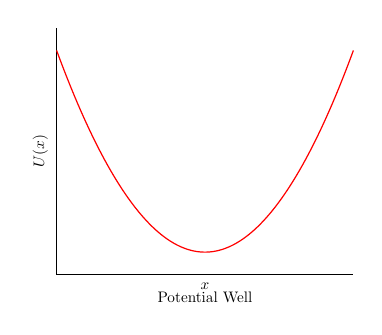
\begin{tikzpicture}[scale=0.55]
            \begin{axis}[
                axis lines=left,
                xlabel=$x$,
                ylabel=$U(x)$,
                ymin=-1, ymax=10,
                xtick=\empty, ytick=\empty,
                axis line style={-},
                clip=false
            ]
            \addplot [
                domain=-3:3,
                samples=100,
                color=red,
                thick,
            ]
            {x^2};
            \node at (axis cs:0, -2) {Potential Well};
            \end{axis}
        \end{tikzpicture}
        \end{minipage}
        \begin{minipage}{0.4\textwidth}    
        \begin{tikzpicture}[scale=0.55]
            \begin{axis}[
                axis lines=left,
                xlabel=$x$,
                ylabel=$P(x)$,
                ymin=0, ymax=1.25,
                xtick=\empty, ytick=\empty,
                axis line style={-},
                clip=false
            ]
            \addplot [
                domain=-3:3,
                samples=100,
                color=blue,
                thick,
            ]
            {exp(-x^2)};
            \node at (axis cs:0, -0.25) {Stationary PDF};
            \end{axis}
        \end{tikzpicture}
        \end{minipage}
    \end{center}
    \end{exampleblock}

\subsection{Special Cases of the Fokker-Planck Equation}

\subsubsection{Deterministic Systems with Random Initial Conditions}
Suppose we have a deterministic system, $\dot{x} = a(x)$, but where the initial conditions are described by a probability distribution $\theta(x)$. Here, randomness comes only from the initial condition, not from noise in the dynamics: the diffusion coefficient is zero, $b(x)=0$. The Fokker-Planck equation loses its second-order derivative term and becomes the \textbf{Liouville equation}:
\small
$$
\begin{cases}
    \dfrac{\partial P(x,t)}{\partial t} = -\dfrac{\partial}{\partial x}\left(a(x)P(x,t)\right) \\[0.8em]
    P(x,0) = \theta(x)
\end{cases}
$$
\normalsize
This type of problem appears, for example, when studying the evolution of a population's distribution over time under deterministic laws, but starting from a known initial distribution.

\subsubsection{Purely Diffusive Systems}
The opposite case occurs when $a(x)=0$, and the system is governed only by noise:
$$
dx = b(x)dW
$$
In population dynamics, this is useful in cases where the baseline growth rate is zero ($r=0$) or constant. In this situation, the Fokker-Planck equation becomes a pure diffusion equation:
$$
\partial_t P = \partial_x^2 \left( \frac{b(x)^2}{2} P(x,t) \right)
$$
This is, in fact, a generalization of the process for the Wiener process, which I recall is $\dot{w} = \xi(t)$ (i.e., $a=0, b=1$). Indeed, using the Fokker-Planck equation, we can find the expression for the PDF of the Wiener process, which will be:
$$
\partial_t P = \frac{1}{2} \partial_w^2 P
$$
Or, analogously, for $\dot{x} = \omega\xi(t)$, which corresponds to the overdamped Brownian motion:
$$
\partial_t P = \frac{\omega^2}{2} \partial_x^2 P
$$

\subsubsection{The Probability Current}
The Fokker-Planck equation can also be viewed in a different way. Given the formula:
\small
$$
\partial_t P = \partial_x \left[ -a(x)P(x,t) - \partial_x \left( \frac{b(x)^2}{2}P(x,t) \right) \right]
$$
\normalsize
If we pull the outer $\partial_x$ out and name the term inside the square brackets $J$, we get:
$$
\partial_t P + \partial_x J = 0
$$
which is the continuity (or flux) equation; in the multi-dimensional case, it is typically written as:
$$
\partial_t \eta + \nabla \cdot J = 0
$$
This makes intuitive sense: if we think of probability as a "substance" (like a population density $\eta$), the change in its distribution is nothing more than a redistribution, so the total amount does not change. The 1D equation found above is easily reduced from the multi-D form of the flux equation. If we take Brownian motion as an example, then:
$$
J = -K \nabla P
$$
For this reason, $J$ in these cases is also known as the \textbf{current}.